\section{Ejemplos}
\label{sec: ejemplos}

\TODO{Como esto es muy importante, deberías hacer esta sección un capítulo;
para no romper con el flujo de la redacción, deberías de mover
más abajo este texto. Para ello, deberías de checar las secciones de abajo
no pongan referencias a esta!}

Definidas ya las bases de Legendre discretas
para toda dimensión $n$ 
(c.f. definición  
\ref{def: base de Legendre discreta}) y estudiadas algunas de sus 
propiedades, planteemos algunos ejemplos
para constatar en dimensiones concretas algunos de los
resultados demostrados en subsecciones anteriores
y empezar a comprobar la utilidad de estas bases para el 
estudio morfológico de señales finitas.


%Inicio ejemplo 1--------------------------------------------
\begin{ejemplo}
A continuación, mostramos las gráficas de los
elementos de las bases $\cali{L}^{2}$ y $\cali{L}^{3}$.
Para dibujar las gráficas usamos los valores
calculados en la tabla
\ref{formulas explicitas para Ln con n de 2 hasta 6}.

\begin{figure}[H]
	\sidecaption{
	Gráficas de los elementos de $\cali{L}^{2}
	\subseteq \IR^{2}$
	\label{fig: graficas elementos L2}
	}
	\centering
	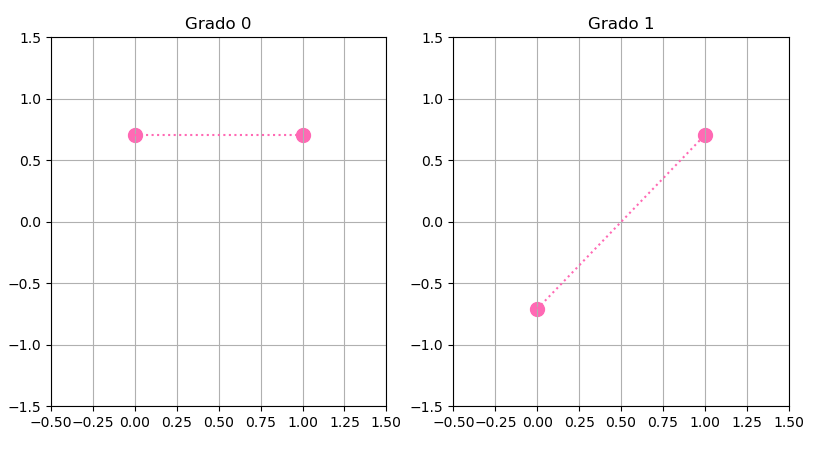
\includegraphics[scale=0.5]{graficasLegendre2} 
\end{figure}	


\begin{figure}[H]
	\sidecaption{
	Gráficas de los elementos de $\cali{L}^{3} 
	\subseteq \IR^{3}$
	\label{fig: graficas elementos L2}
	}
	\centering
	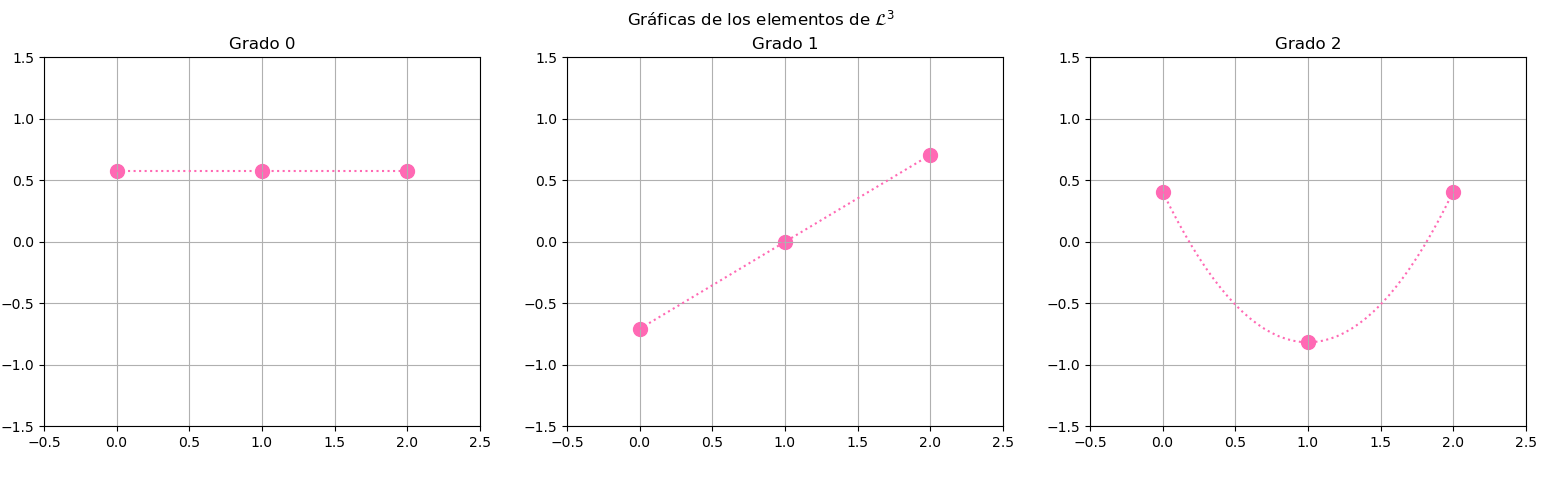
\includegraphics[scale=0.26]{graficasLegendre3} 
\end{figure}	




En el caso $n=2$, el único subespacio de polinomios
discretos no trivial es 
\begin{align*}
W_{2,0}= & span \left\{ 
\left(\frac{1}{\sqrt2}, \frac{1}{\sqrt2} \right) \right\} \\
= & \{ (x,x) \in \IR^{2}: \hspace{0.2cm} x \in \IR \},
\end{align*}

pues

\begin{equation}
\label{eq1: 1Dic}
W_{2,1}= \IR^{2}.
\end{equation}


En el caso $n=3$, calculamos que
\begin{align*}
W_{3,0}= & span \left\{
\left( \frac{1}{\sqrt3}, \frac{1}{\sqrt3},
\frac{1}{\sqrt3} \right) \right\}  \\
= & \{ (x,x,x) \in \IR^{3}: \hspace{0.2cm} x \in \IR \},
\end{align*}

\begin{align}
\label{eq2: 1Dic}
W_{3,1}= & span \left\{ \left( \frac{1}{\sqrt3}, \frac{1}{\sqrt3},
\frac{1}{\sqrt3} \right) ,
\left( -\frac{1}{\sqrt2}, 0,  \frac{1}{\sqrt2} \right) \right\}
\nonumber \\
= & \{ (x,y,2y-x) \in \IR^{3}: \hspace{0.2cm} x,y \in \IR \},
\end{align}
y
\[
W_{3,2}=\IR^{3}.
\]

\begin{figure}[H]
	\sidecaption{
	Gráficas de 
	$W_{2,0} \subseteq \IR^{2}$
	y de los subespacios
	$W_{3,0}$ y $W_{3,1}$ de $\IR^{3}$ que
	son, respectivamente, una recta y un plano;
	observe que
	$W_{3,0} \subseteq W_{3,1}$ y que tanto 
	$W_{2,0}$ como $W_{3,1}$ dividen en dos regiones
	ajenas a sus correspondientes espacios ambiente.
	\label{fig: graficas espacios W para dimensiones 2 y 3}
	}
	\centering
	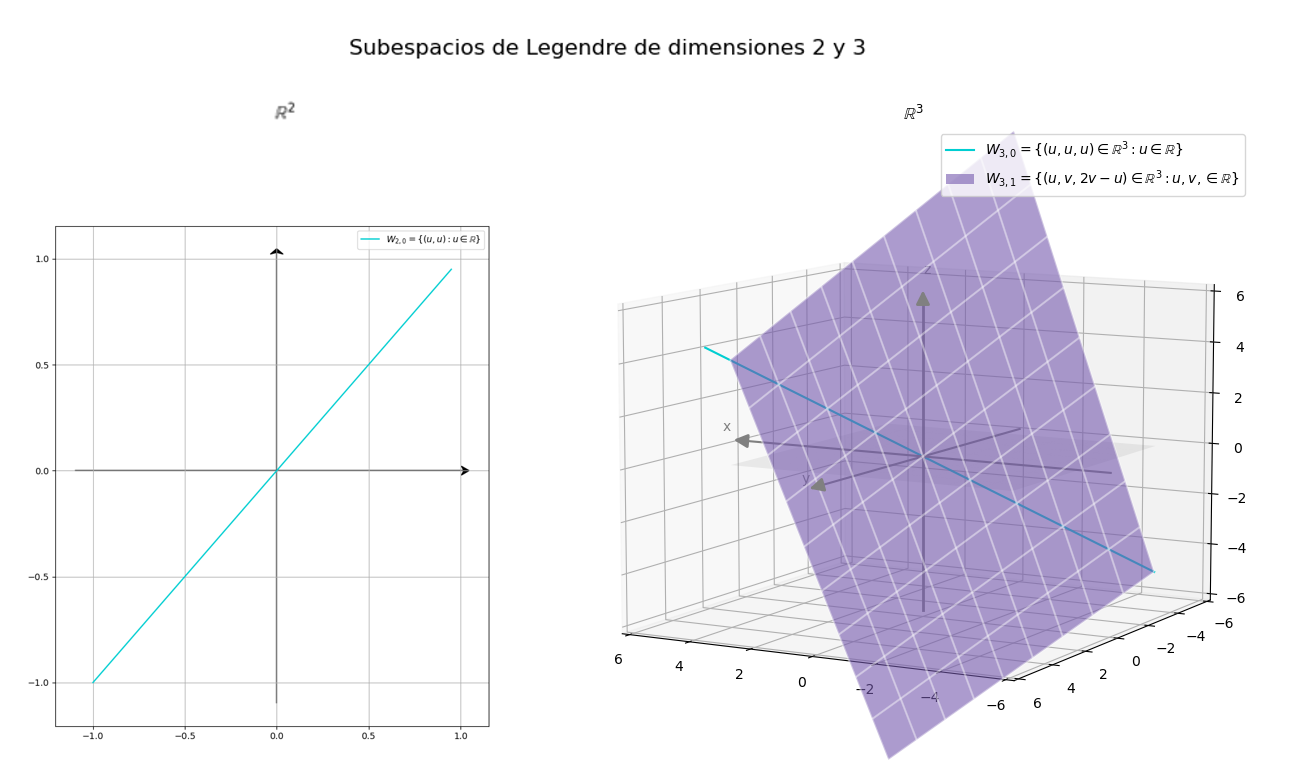
\includegraphics[scale= 0.38]{legendre2y3} 
\end{figure}	
	 
\final
\end{ejemplo}
%final ejemplo 1--------------------------------------------





%Inicio ejemplo 2--------------------------------------------

\begin{ejemplo}
Considere al siguiente conjunto de cinco
puntos del plano:
\begin{equation} \label{eq: conjunto cinco puntos}
\{ (0,-0.5), (1,2.4), (2, 1.6), (3,1.7), (4, 2.3) \}.
\end{equation}


Como tenemos cinco puntos, trabajamos
en el espacio $\IR^{5}$. 
La regresión lineal calculada a partir
del conjunto de datos
\eqref{eq: conjunto cinco puntos}
es la recta
con ecuación cartesiana

\begin{equation} \label{eq: recta minimos cuadrados}
y=0.49x+0.52.
\end{equation}

El vector cuyas entradas
son las cinco mediciones (dadas por las ordenadas
de los puntos del conjunto \eqref{eq: conjunto cinco puntos})
es
\begin{equation}
\label{eq0: 29Nov}
x=(-0.5, 2.4, 1.6, 1.7, 2.3).
\end{equation}


\begin{figure}[H]
	\sidecaption{
	Gráfica de la señal $x \in \IR^{5}$.
	\label{fig: grafica semal x ejemplo}
	}
	\centering
	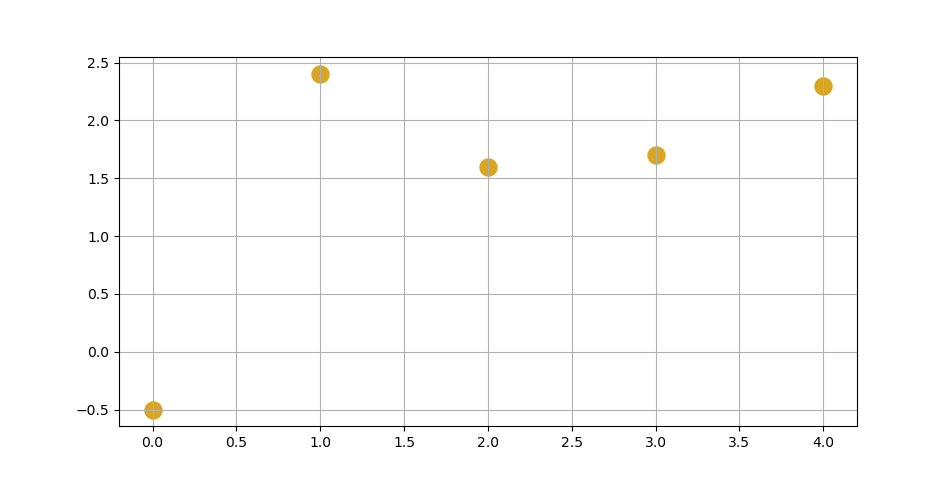
\includegraphics[scale=0.4]{graficaX_31Oct} 
\end{figure}	


Nos interesa
dar explícitamente a 
la señal $\Pi_{W_{5,1}}(x) \in W_{5,1} \leq \IR^{5}$.
En realidad, por ser $\cali{L}^{5}$ 
una base ortonormal de $\IR^{5}$ y por ser
$W_{5,1}$ el subespacio generado por los
dos primeros vectores de esta base, 
se sabe de inmediato que
\[
\Pi_{W_{5,1}}(x)=  \langle \Pi_{W_{5,1}}(x), \cali{L}^{5,0} \rangle \cali{L}^{5,0}
+ \langle \Pi_{W_{5,1}}(x), \cali{L}^{5,1} \rangle \cali{L}^{5,1};
\]
de todas formas, como ilustración, planteemos un sistema
de ecuaciones para llegar a una expresión para
$\Pi_{W_{5,1}}(x)$.
Usando las expresiones para los vectores
de $\cali{L}^{5}$
dadas en \ref{subsect:Formulas explicitas},
tenemos que
\[
W_{5,1}=span\{ (1,1,1,1,1,1), (-2, -1, 0, 1, 2) \},
\]

y 
\[
W_{5,1}^{\perp}=span\{ (2,-1,-2,-1,2), (-1,2,0,-2,1), (1,-4,6,-4,1)\}.
\]
Según el teorema de la proyección ortogonal \ref{Teo:proyOrt},
$\Pi_{W_{5,1}}(x)$ es el único elemento de $W_{5,1}$ para el 
que 

\[
x-\Pi_{W_{5,1}}(x) \in W_{5,1}^{\perp};
\]
esto se 
traduce en la existencia de 
únicos escalares $c_{1}$, $c_{2}$,
$a_{1}$, $a_{2}$ y $a_{3}$ tales que
\[
x-c_{1}(1,1,1,1,1)-c_{2}(-2, -1, 0, 1, 2)
\]
es igual a 

\[
a_{1}(2,-1,-2,-1,2)+a_{2}(-1,2,0,-2,1)
+ a_{3}(1,-4,6,-4,1),
\]
\noindent
o sea, tales que

\begin{equation*}
\begin{cases}
-0.5-(c_{1}-2c_{2})=2a_{1}-a_{2}+a_{3}, \\
2.4-(c_{1}-c_{2})=-a_{1}+2a_{2}-4a_{3}, \\
1.6-c_{1}=-2a_{1}+6a_{3},\\
1.7-(c_{1}+c_{2})=-a_{1}-2a_{2}-4a_{3}, \\
2.3-(c_{1}+2c_{2})=2a_{1}+a_{2}+a_{3}.
\end{cases}
\end{equation*}
Resolviendo este sistema
de ecuaciones, encontramos que
$c_{1}=1.5$ y $c_{2}=0.49$. Así,




\begin{align}
\label{eq5: 23Oct}
\Pi_{W_{5,1}}(x) =& c_{1} (1,1,1,1,1) + c_{2}(-2-1,0,1,2) \nonumber \\
= & (0.52, 1.01, 1.5, 1.99, 2.48 );
\end{align}
observe que \eqref{eq5: 23Oct} es, 
en efecto, la discretización de 
la recta \eqref{eq: recta minimos cuadrados}
en la malla uniforme $\cali{P}_{5}$.
De forma análoga se calcula la parte cuadrática de
la señal $s$.

\begin{figure}[H]
	\sidecaption{
	Gráficas de $x$, 
	$\Pi_{W_{5,0}}(x)$, $\Pi_{W_{5,1}}(x)$ y $\Pi_{W_{5,2}}(x)$.
	\label{fig: partes afin, lineal y cuadratica} 
	}
	\centering
	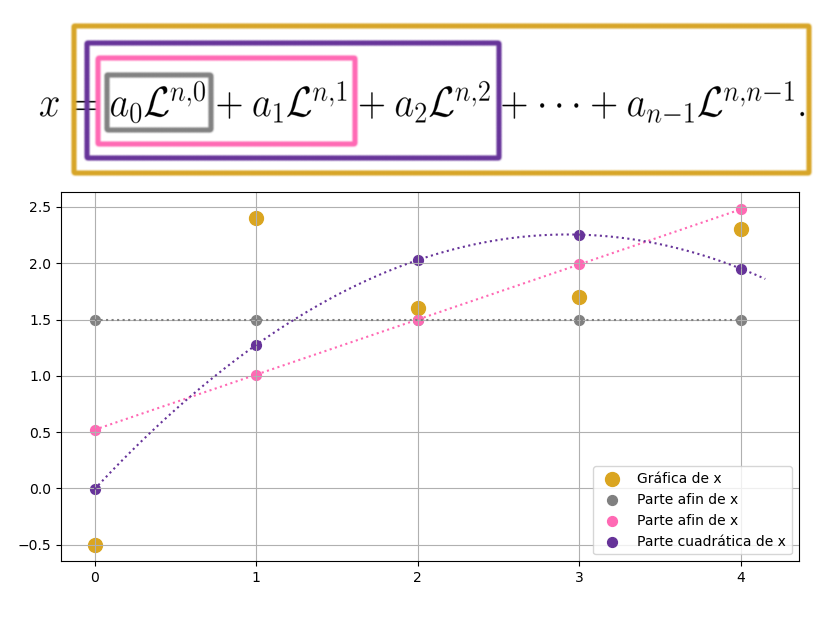
\includegraphics[scale=0.6]{parteAfinCuadr}
\end{figure}	
\final
\end{ejemplo}
%Final ejemplo 2--------------------------------------------


\TODO{Sería bueno notar que estas dando un
algoritmo de transformación de la raw data
via una proyección lineal (proceso mediante
en cual se destruye información). Nada de ML, 
esto es más bien symbolic AI (deep learning with
python, p.35)}



En el siguiente ejemplo 
damos dos propuestas naturales,
usando los espacios de polinomios discretos $W_{n,k}$,
para poder dar no sólo respuestas del tipo
``sí/no'' a preguntas sobre la morfología de una señal, sino,
de forma más general, del tipo ``qué tanto sí'' o
``qué tanto no''.



%Inicio ejemplo 3--------------------------------------------

\begin{ejemplo}
Sea $x \in \IR^{n}$. Digamos que 
\[
x = \suma{k=0}{n-1}{a_{k} \cali{L}^{n, k}}.
\]


Como se argumentó ya, las proposiciones
\begin{center}
``$x \in \IR^{n}$ es afín'' \hspace{0.2cm} y \hspace{0.2cm} 
``$x \in W_{n,1}$''
\end{center} 
son equivalentes.
Observe que, aún cuando no se cumpla el caso
extremos de que $x$ sea elemento 
de $W_{n,1}$ (y, por lo tanto, no podamos aseverar que
$x$ es afín), provistos
de nociones como las de norma y ortogonalidad, es fácil dar 
una propuesta legítima de
\textbf{medidas} de ``qué tan afín'' es la señal $x$,
o, en términos matemáticos, de qué tanto se aleja
$x$ del espacio de señales afines de su correspondiente
espacio ambiente.

Como se argumentó en la subsección \ref{cosine similarity}, hay
dos formas plausibles de dar medidas de qué tan cerca está
$x$ del plano $W_{n,1}$;

\begin{itemize}
\item[a)] Una forma obvia de proceder es calcular la norma
del vector 
\[
x - \Pi_{W_{3,1}}(x)= \suma{k=2}{n-1}{a_{k} \cali{L}^{n, k}},
\]
es decir, tomar al número no negativo
\[
\sqrt{ \suma{k=2}{n-1}{a_{k}^{2}}}
\]
como una medida de qué tanto se aleja $x$ del plano $W_{n,1}$
(o sea, de qué tanto se aleja $x$ de ser afín).

\item[b)] Otro acercamiento podría ser preguntarse por
el ángulo $\alpha \in [0, \frac{\pi}{2}]$ 
que forma el vector $x$ con
$W_{n,1}$, el espacio de señales afines $n-$dimensionales.
\end{itemize}
Veamos por qué la segunda (la que corresponde a medir
el ángulo que forma $x$ con su proyección al espacio de señales afines)
es la mejor forma de proceder.

Si $x \in \IR^{n}$ es una señal de dimensión $n$ y 
$a \in \IR-\{ 0 \}$ es un escalar cualquiera,
la gráfica de $a \cdot x$ no es más que la gráfica 
de $x$ reescalada por un factor de $a$ cuando este
último es positivo; en caso contrario, es la gráfica
de $x$ reescalada pero además reflejada respecto al eje
horizontal.

La morfología de la gráfica de $x$ es entonces,
salvo reflexiones horizontales, invariante bajo multiplicación
escalar; otro atributo de $x$ que no se ve afectado por esta acción
es el ángulo que forma con el plano $W_{n,1}$ de señales afines
(c.f. proposición \ref{prop: angulo se conserva bajo mult. esc.}), 
aunque la distancia euclidea de la señal
al plano $W_{n,1}$ por lo general sí es afectada por multiplicaciones escalares.


\begin{figure}[H]
	\sidecaption{ Para $n=3$,
	se grafica a $x$ junto con algunos múltiplos escalares de $x$.
	Observe que, salvo reflexiones horizontales, la gráfica de estas
	señales tiene la misma forma.
	\label{fig: aaa} 
	}
	\centering
	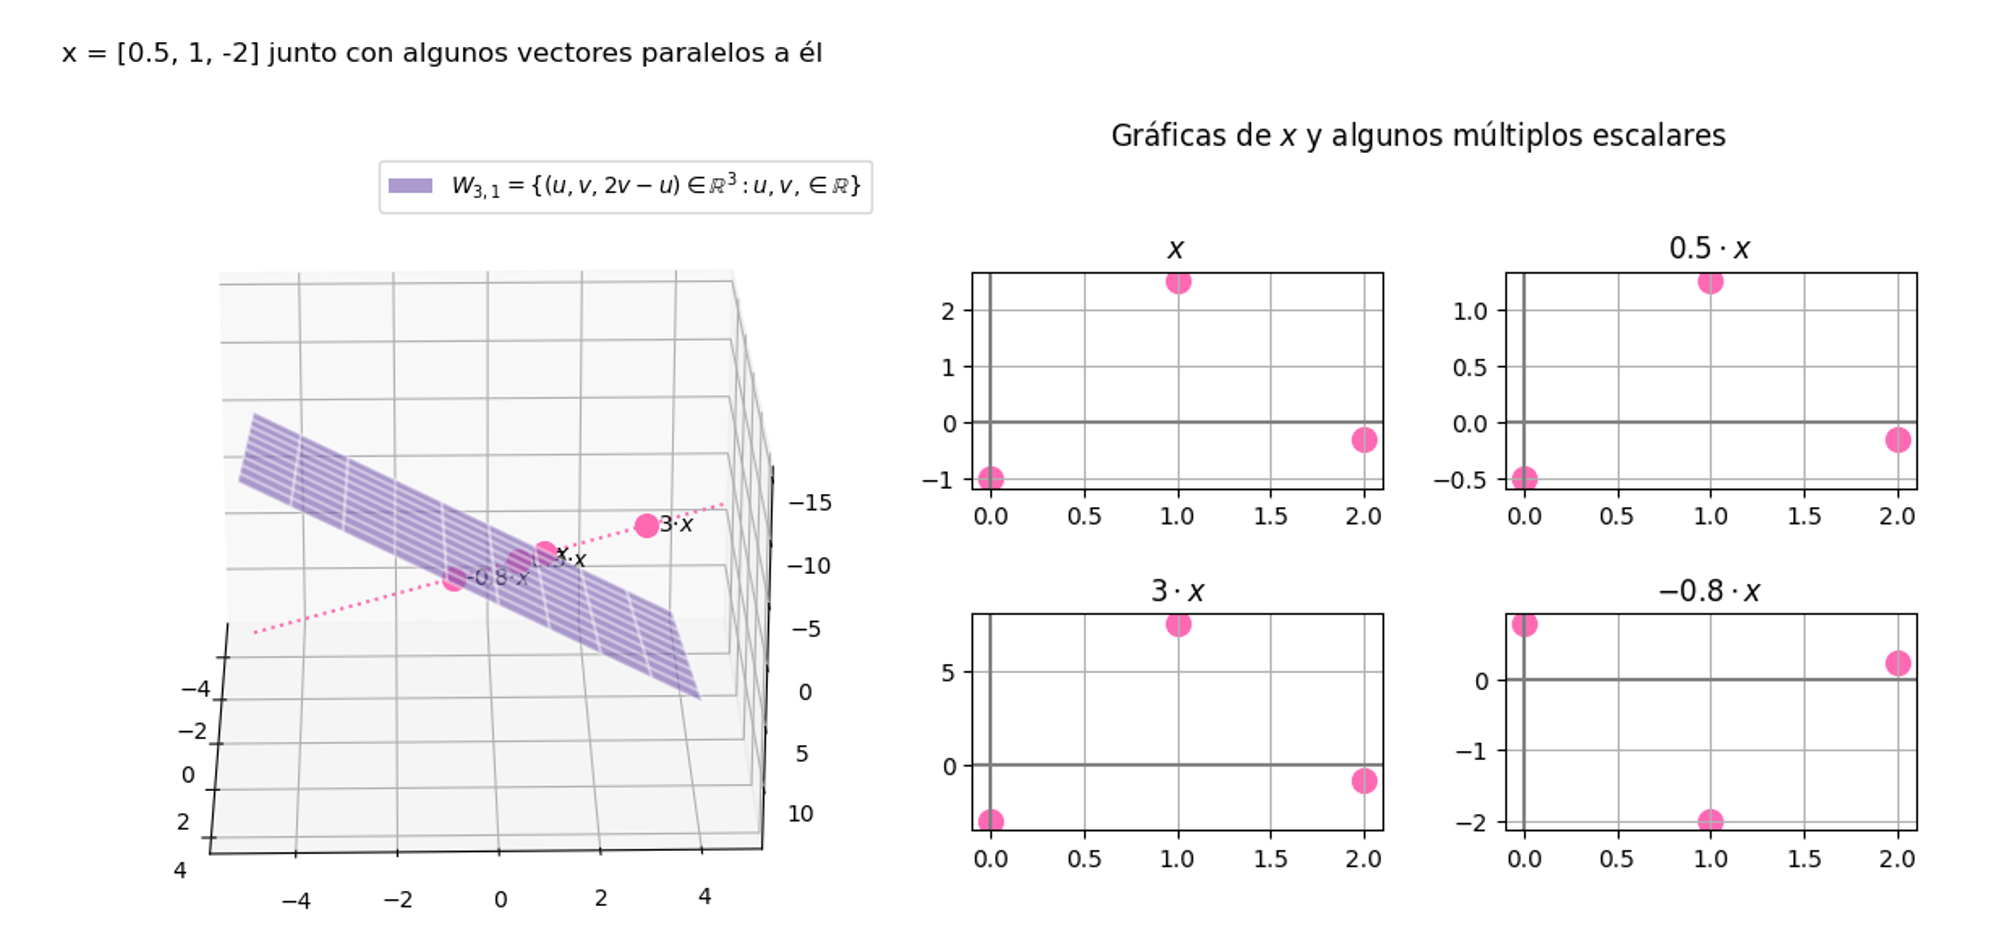
\includegraphics[scale=0.18]{borrador}
\end{figure}

\textbf{Tomamos pues al coseno del ángulo que forma $x$ con su proyección
al plano $W_{n,1}$ como una medida de cercanía de $x$ a la propiedad de 
ser afín.}


Para dar un ejemplo concreto, fijemos $n=3$.
Como se calculó en \eqref{eq2: 1Dic},
el subespacio $W_{3,1} \leq \IR^{3}$ de señales afines es el plano
de ecuación cartesiana

\[
W_{3,1}: \hspace{0.2cm} x-2y+z=0.
\]
Sea 
\begin{equation*}
\label{eq0: 9Feb}
x=a_{0}\cali{L}^{3,0}+a_{1}\cali{L}^{3,1}+a_{2}\cali{L}^{3,2}
\end{equation*}
un vector del espacio.


Como las dimensiones de $\IR^{3}$ y $W_{3,1}$ 
difieren por uno,
este útimo es un hiperplano
\sidenote{Puede recordar la definición
de hiperplano en 
\ref{section: hiperplanos}.}
del primero; como $\cali{L}^{3,2}$
es un vector normal a $W_{3,1}$
(c.f. corolario \ref{cor: Ln,k ortogonal a todo pol discreto de grado menor a k}), 
si $\varphi: \IR^{3} \longrightarrow \IR$ es la función
definida como
\begin{equation}
\label{eq: funcion phi ejemplo}
\varphi(x)= \langle \cali{L}^{3,2} , x \rangle =a_{2},
\end{equation}



las tres regiones ajenas en las
que $W_{3,1}$ divide al espacio
$\IR^{3}$ son 


\begin{itemize}
\item[I)] $\{ x \in \IR^{3} : \varphi(x)>0 \}$,
región a la que pertenece $\cali{L}^{3,2}$,
\item[II)] $W_{3,1}= Ker(\varphi)$, y 
\item[III)] $\{ x \in \IR^{3} : \varphi(x)<0 \}$,
región a la que pertenece $-\cali{L}^{3,2}$.
\end{itemize}

\begin{figure}[H]
	\sidecaption{Se ilustran las tres 
		regiones en las que $W_{3,1} \subseteq \IR^{3}$ divide al espacio,
		clasificadas según el signo que tome 
		la función $\varphi$ como se definió en
		\eqref{eq: funcion phi ejemplo}. En
		{\color{ameDorado}{dorado}} se muestra al vector
		$\cali{L}^{3,2}$, en {\color{ameRosa}{rosa}}
		un elemento de la región citada, y en 
		{\color{ameMorado}{morado}} la proyección de este
		al espacio $W_{3,1}$.
	\label{fig: angulo x y proy} 
	}
	\centering
	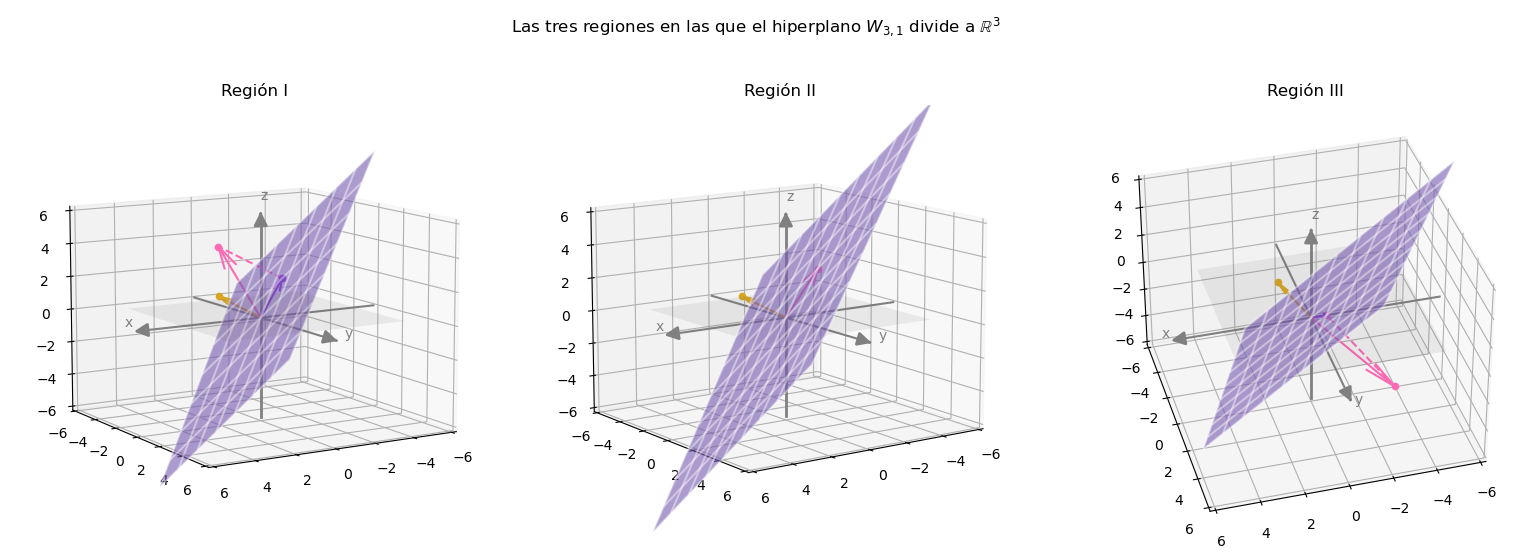
\includegraphics[scale=0.3]{2Dic_4} 
\end{figure}

Es fácil obtener una expresión para el coseno del ángulo
$\alpha$ en términos de los coeficientes de $x$ respecto a $\cali{L}^{3}$:

\begin{figure}[H]
	\sidecaption{Encontrando una fórmula explícita del 
	ángulo que forma $x$ con $\Pi_{W_{3,1}}(x)$.
	\label{fig: angulo x y proy} 
	}
	\centering
	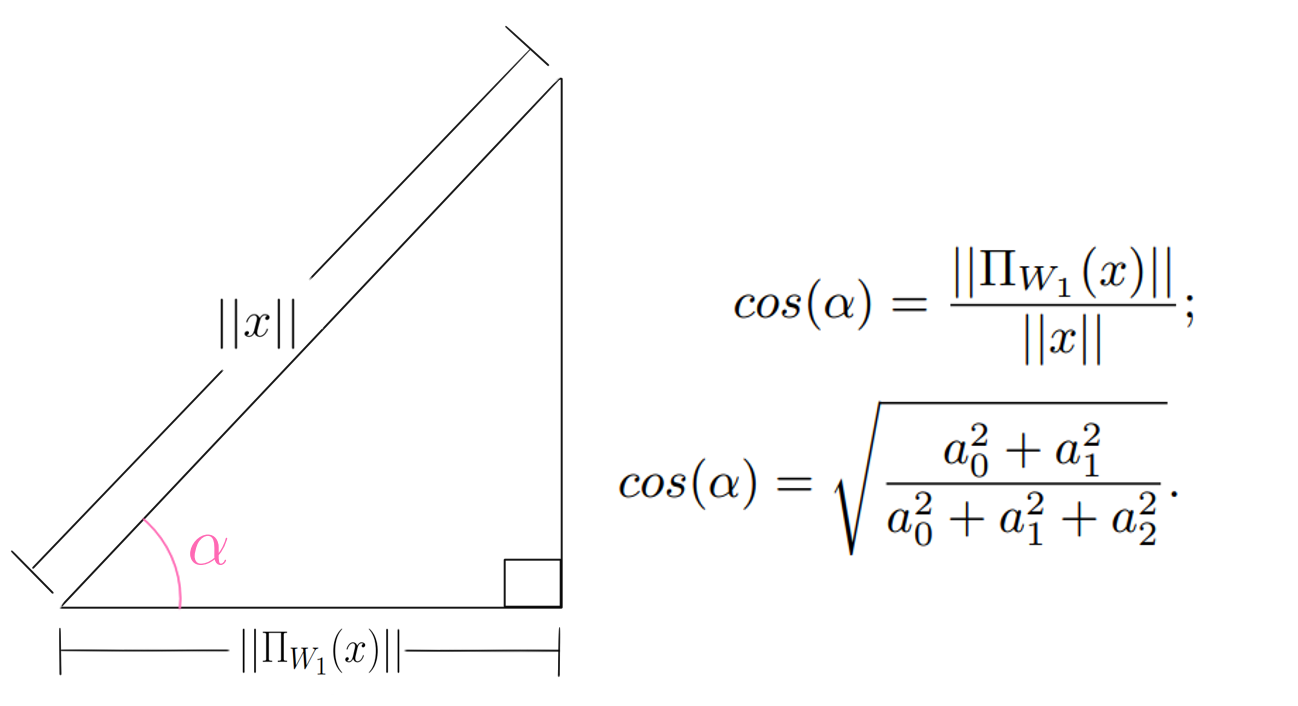
\includegraphics[scale=0.7]{2Dic_3}
\end{figure}


De las relaciones de la figura 
\ref{fig: angulo x y proy} 
obtenemos una igualdad que relaciona el ángulo 
$\alpha$ que forma una señal $x \in \IR^{3}$ 
con su proyección al espacio $W_{3,1}$
con los coeficientes $a_{i}$
de $x$ respecto a $\cali{L}^{3}$:
\begin{equation}
\label{eq0: 3Dic}
cos(\alpha)= \sqrt{\frac{a_{0}^{2}+a_{1}^{2}}{a_{0}^{2}+a_{1}^{2}+a_{2}^{2}}}.
\end{equation}

Para un ejemplo aún más concreto, hagamos 
\begin{equation}
\label{eq1: 19Sept}
a_{0}= \sqrt{3}, \hspace{0.2cm} a_{1}= \sqrt{2},
\end{equation}


\noindent
es decir, consideremos a todos los vectores de $\IR^{3}$
cuya proyección al plano $W_{3,1}$ es 
el vector
\begin{equation}
\label{eq1: 6Dic}
(0,1,2).
\end{equation}
Es obvio que el conjunto de los puntos
del espacio cuya proyección a
$W_{3,1}$ es \eqref{eq1: 6Dic} de hecho la recta
con ecuación vectorial
\begin{equation}
\label{eq0: 6Dic}
l_{(0,1,2)} := (0,1,2)+c(1,-2,1), \hspace{0.2cm} c \in \IR.
\end{equation}

\noindent
Sustituyendo
los valores \eqref{eq1: 19Sept} en \eqref{eq0: 3Dic} y
despejando
\sidenote{
En general, si $C:= || \Pi_{W_{3,1}}(x) || ^{2}$,
entonces $a_{2}^{2}= C \cdot4 tg^{2}(\alpha).$
}, obtenemos 
\[
|a_{2}|= \sqrt{5 tg^{2}(\alpha)};
\]
el signo del coeficiente $a_{2}$ (que corresponde a la dirección
de $\cali{L}^{3,2}$ en la descomposición de $x$) se determina por
la región en la que se encuentre $x$;

\begin{itemize}
\item el signo de $a_{2}$ es positivo si $x$ es elemento de la región I,
\item $a_{2}=0$ si $x$ es elemento de la región II, y
\item el signo de $a_{2}$ es negativo si $x$ es elemento de la región III.
\end{itemize}


Grafiquemos ahora algunos elementos
de la recta \eqref{eq0: 6Dic}.
Los valores de las entradas de $x$, en la
mayoría de los casos, han sido redondeados.


\begin{figure}[H]
	\sidecaption{Aquí se considera al vector 
		$x$ que forma un ángulo $\alpha=\pi/3$
		con el plano $W_{3,1}$ y que se ubica en la región I.
	\label{fig: angulo x y proy} 
	}
	\centering
	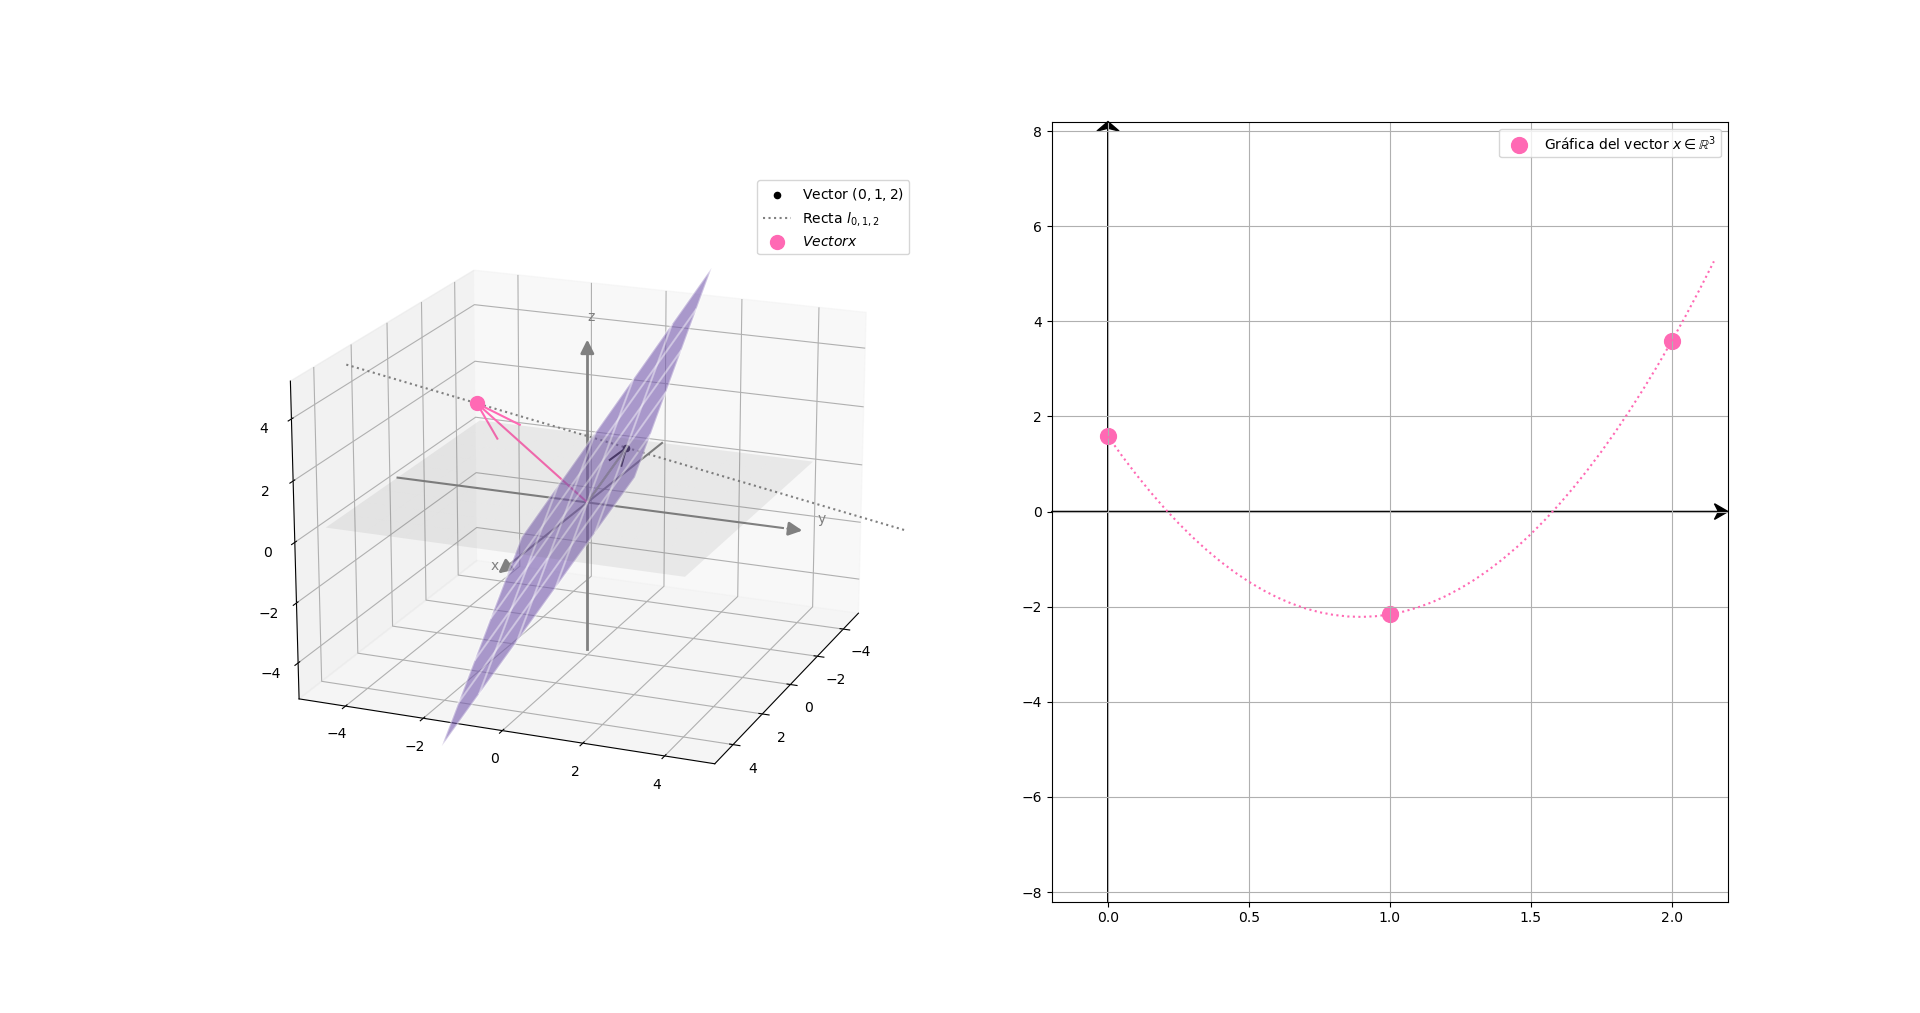
\includegraphics[scale=0.3]{6Dic_0}
\end{figure}



\begin{figure}[H]
	\sidecaption{Aquí se considera al vector 
		$x$ que forma un ángulo $\alpha=\pi/3$
		con el plano $W_{3,1}$ y que se ubica en la región I.
	\label{fig: angulo x y proy} 
	}
	\centering
	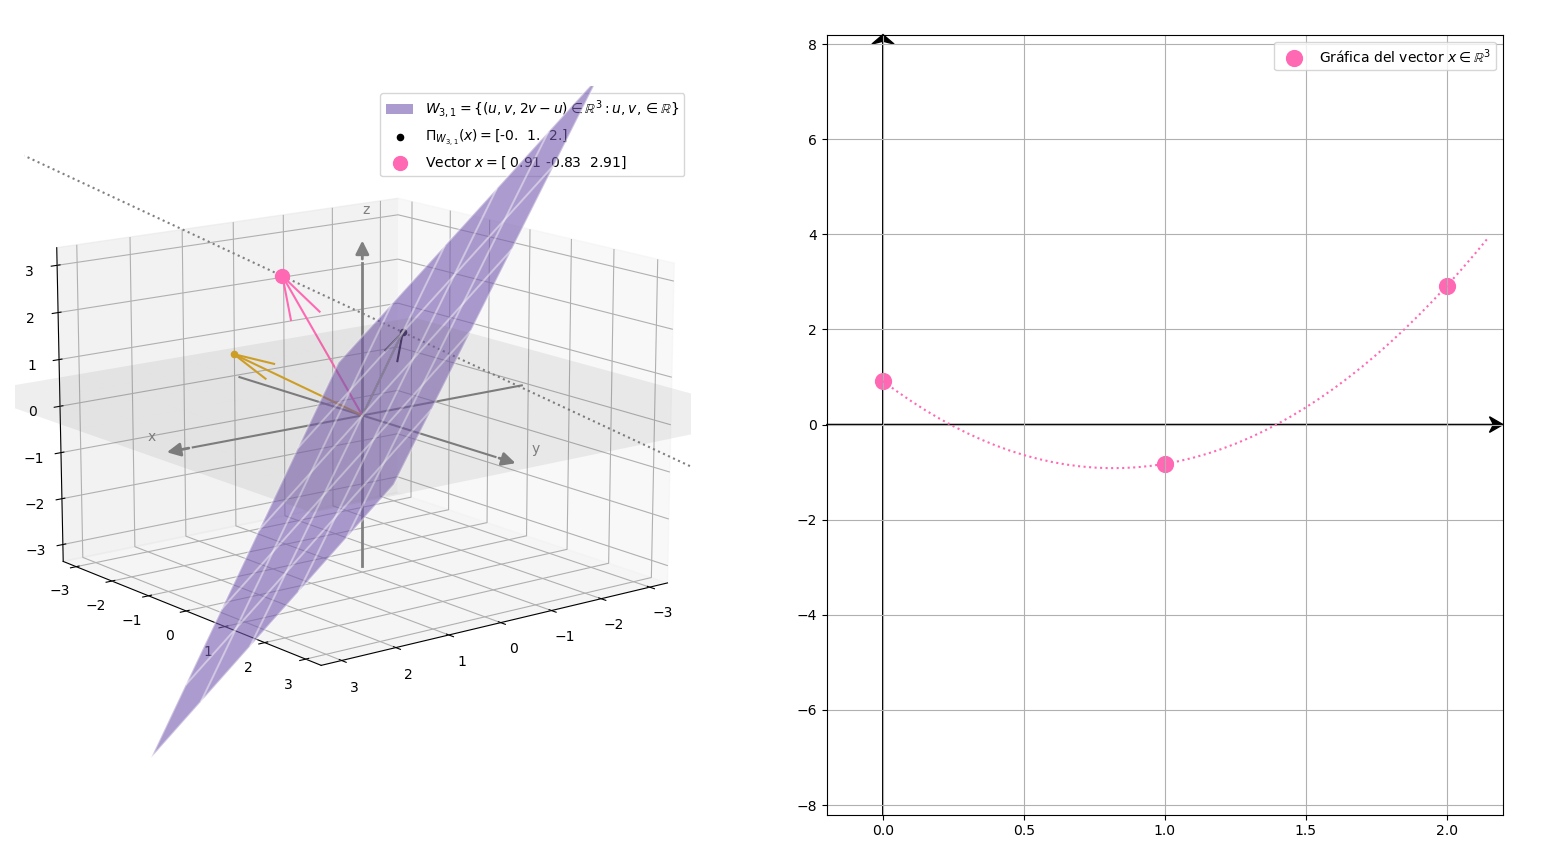
\includegraphics[scale=0.3]{6Dic_1}
\end{figure}

\begin{figure}[H]
	\sidecaption{Aquí se considera al vector 
		$x$ que forma un ángulo $\alpha=0$
		con el plano $W_{3,1}$ y que se ubica en la región II.
	\label{fig: angulo x y proy} 
	}
	\centering
	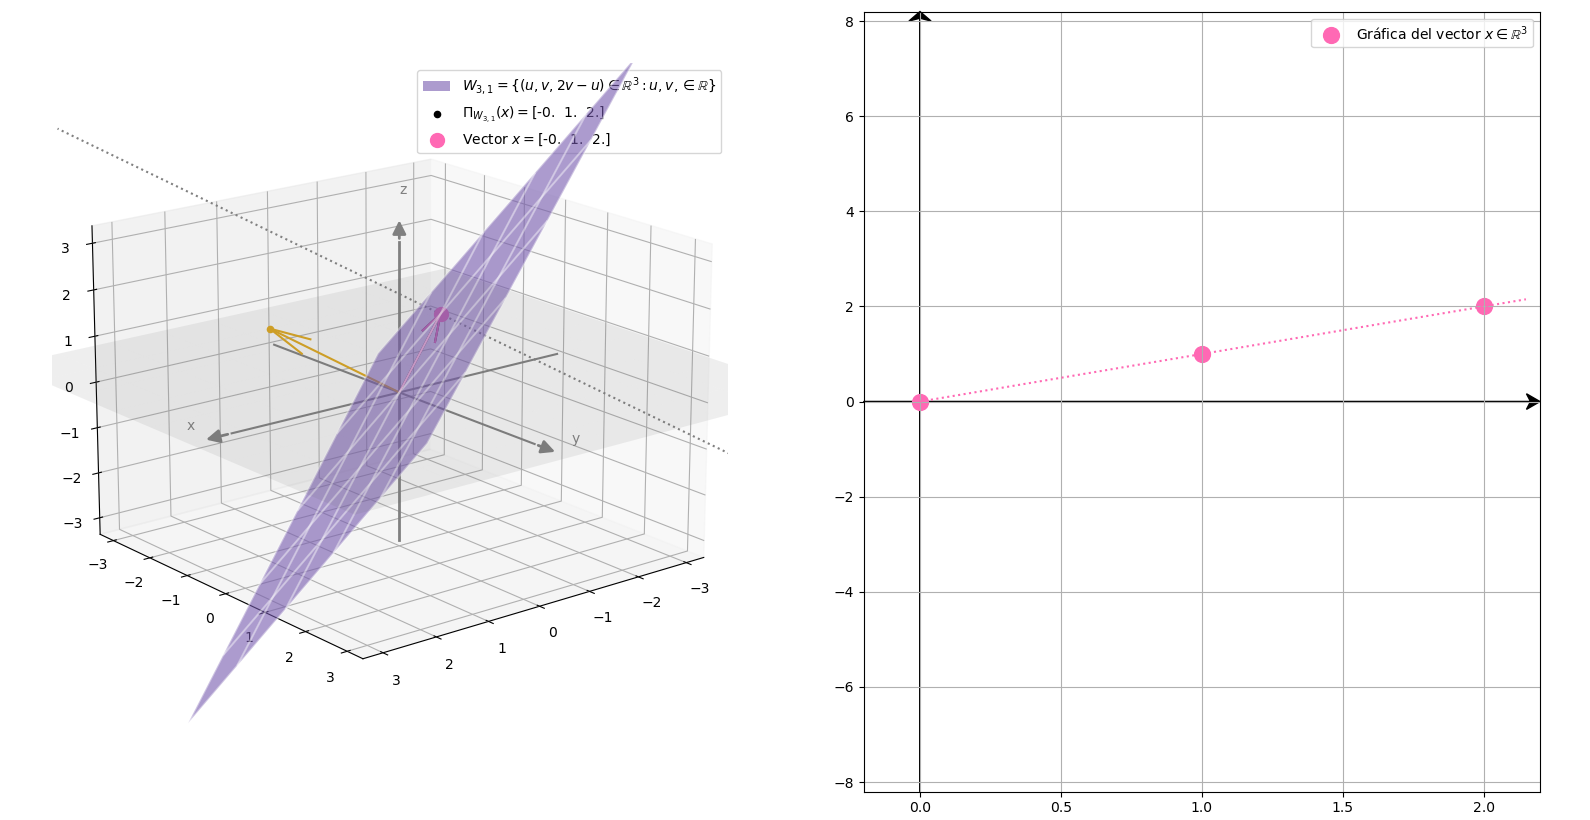
\includegraphics[scale=0.3]{6Dic_2}
\end{figure}

\begin{figure}[H]
	\sidecaption{Aquí se considera al vector 
		$x$ que forma un ángulo $\alpha=\pi/3$
		con el plano $W_{3,1}$ y que se ubica en la región III.
	\label{fig: angulo x y proy} 
	}
	\centering
	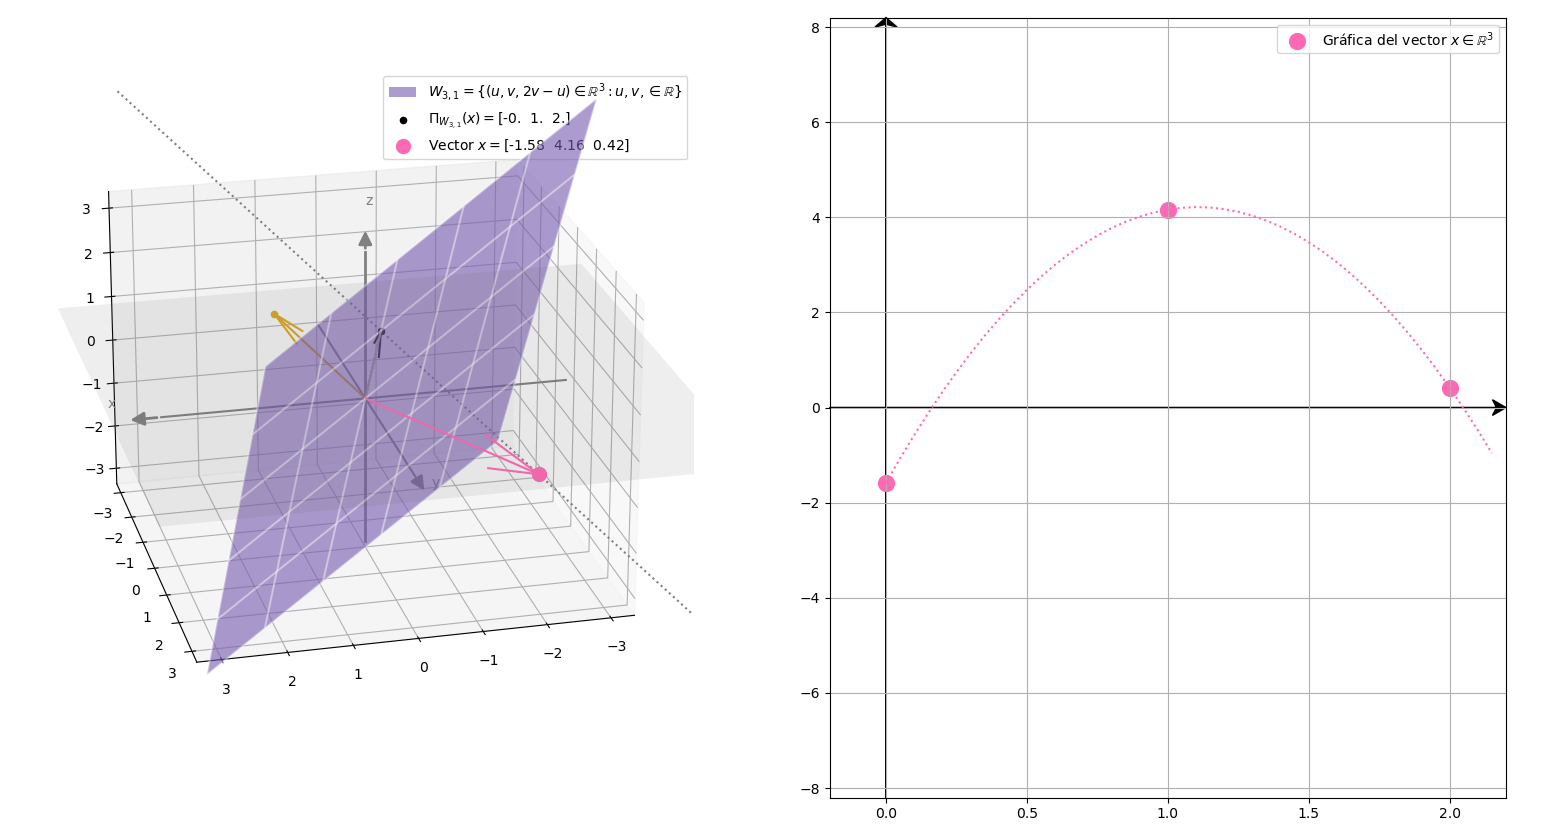
\includegraphics[scale=0.3]{6Dic_3}
\end{figure}

\begin{figure}[H]
	\sidecaption{Aquí se considera al vector 
		$x$ que forma un ángulo $\alpha=6\pi/17$
		con el plano $W_{3,1}$ y que se ubica en la región III.
	\label{fig: angulo x y proy} 
	}
	\centering
	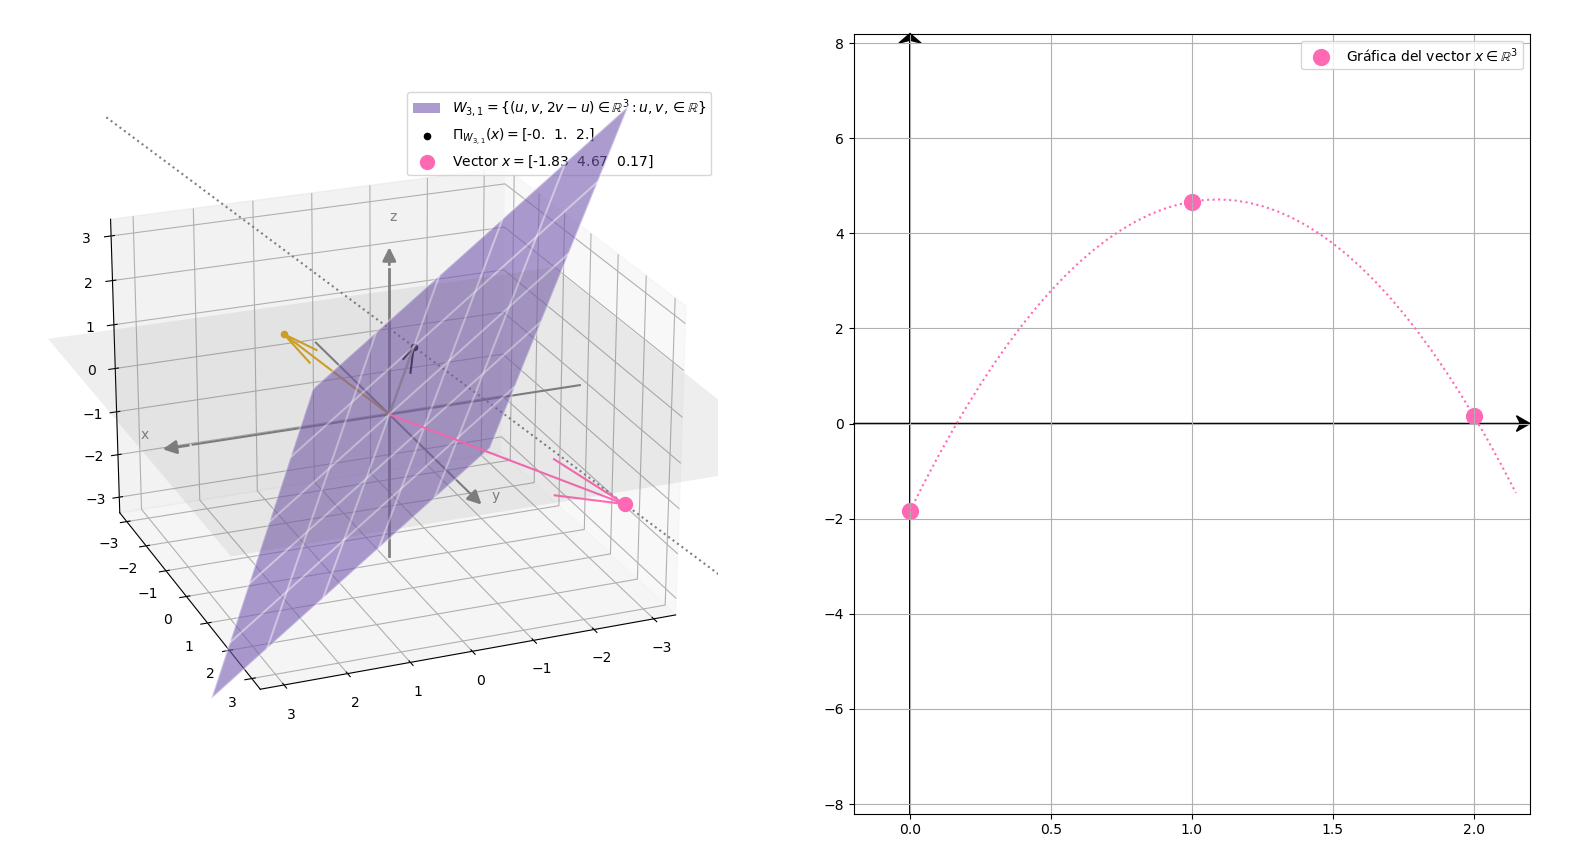
\includegraphics[scale=0.3]{6Dic_4}
\end{figure}


\final
\end{ejemplo}
%Final ejemplo 3--------------------------------------------
